\capitulo{4}{Metodología}
\label{cap:metodologia}


La metodología seguida en este proyecto abarca todas las fases del desarrollo de un sistema predictivo de trastornos del sueño, con un enfoque ingenieril aplicado al ámbito clínico, que prioriza tanto la utilidad predictiva como la interpretabilidad. Se parte del tratamiento inicial de los datos, pasando por la evaluación y selección del modelo más adecuado, hasta el despliegue en una aplicación interactiva accesible para profesionales sanitarios o usuarios interesados. A continuación, se describen en detalle las etapas y técnicas empleadas.

\section{Desarrollo del modelo predictivo}

Para la implementación del modelo predictivo y su posterior integración en una aplicación interactiva, se utilizaron diversas herramientas y tecnologías que permitieron abarcar el proyecto desde el tratamiento de datos hasta el desarrollo de la interfaz.

Además de buscar un alto rendimiento estadístico, el objetivo fue desarrollar un sistema útil en el contexto clínico, capaz de proporcionar predicciones explicables sobre la presencia o ausencia de trastornos del sueño, facilitando su uso por parte de profesionales o usuarios sin conocimientos técnicos.

A continuación, se describen en detalle las etapas de análisis, entrenamiento y evaluación del sistema.


\subsection{Descripción de los datos}
El modelo predictivo desarrollado en este proyecto se ha basado en un conjunto de datos de acceso público, descargado de la plataforma \textbf{\href{https://www.kaggle.com/}{Kaggle}},  especializada en ciencia de datos y aprendizaje automático. El dataset seleccionado, titulado Sleep Health and Lifestyle Dataset\footnote{Dataset seleccionado: \cite{alnour2024kaggle}}, proporciona información sociodemográfica, clínica y de hábitos de vida de un total de 374 individuos.

Este conjunto de datos tiene como finalidad facilitar el estudio computacional de los principales trastornos del sueño mediante el análisis conjunto de factores personales, fisiológicos y conductuales, ofreciendo así una perspectiva multidimensional alineada con enfoques clínicos actuales.

Las variables incluidas en el conjunto de datos se pueden agrupar de la siguiente manera:
\begin{itemize}
    \item \textbf{Variables demográficas:}
\begin{itemize}
    \item Age: edad del paciente, expresada en años.
    \item Gender: género biológico, bien sea masculino o femenino (Male/Female).
    \item \textit{Occupation:} ocupación laboral principal (ingeniero, médico, representante de ventas...).
\end{itemize}

\item  \textbf{Variables clínicas:}
\begin{itemize}
    \item \textit{Blood Pressure}: presión arterial registrada en formato sistólica/diastólica, medida en mmHg ("120/80").
    \item  \textit{Heart Rate}: frecuencia cardíaca en reposo, representada en latidos por minuto.
    \item  \textit{BMI Category}: clasificación del índice de masa corporal (Underweight, Normal, Overweight, Obese)
\end{itemize}

  \item \textbf{Variables conductuales y de estilo de vida:}
\begin{itemize}
    \item Sleep Duration: duración media del sueño, en horas.
\item Quality of Sleep: valoración subjetiva de la calidad del sueño, incluida en una escala comprendida entre el 1 y el 10.
\item \textit{Stress Level}: nivel de estrés al que se ve sometido el paciente, percibido por él mismo. Representado en una escala del 1 a 10.
\item \textit{Physical Activity Level}: nivel de actividad física semanal (valor de 0 a 100). 
\item \textit{Daily Steps}: número medio de pasos diarios.
\end{itemize}
\item \textbf{Variable objetivo (target):}
\begin{itemize}
    \item \textit{Sleep Disorder}: clasificación del trastorno del sueño, categorizado en tres clases:
    \begin{itemize}
        \item \textit{None}: sin trastorno diagnosticado.
        \item \textit{Insomnia}: diagnóstico de insomnio.
        \item \textit{Sleep Apnea}: diagnóstico de apnea del sueño.
    \end{itemize}
\end{itemize}
\end{itemize}

El dataset original se encuentra en formato CSV (valores separados por comas) y fue tratado íntegramente en \textbf{Python}, utilizando librerías especializadas como \textbf{Pandas} y \textbf{NumPy} para su carga, transformación, análisis y modelado.

Aunque el conjunto de datos presenta limitaciones propias de los datos sintéticos o autodeclarados (como posibles sesgos o simplificaciones de la realidad clínica), su estructura es adecuada para la experimentación y la validación de metodologías de aprendizaje automático en el ámbito de la salud.

El conjunto de datos utilizado puede consultarse en el siguiente enlace: 
\href{https://www.kaggle.com/code/alnourabdalrahman9/sleeping-disorders-detection-outliers-removal/input}{\texttt{Sleep\_health\_and\_lifestyle\_dataset.csv}.}

\subsection{Carga y descripción inicial del conjunto de datos}

El archivo original fue cargado en un entorno de \href{file://C:/Users/Marina/OneDrive\%20-\%20Universidad\%20de\%20Burgos/Escritorio/TFG-Marina-Martin/notebooks/TFG3-Marina.ipynb}{Jupyter Notebook} mediante la librería \textbf{Pandas}, utilizando estructuras tipo \textbf{DataFrame}. Esta organización permitió realizar de forma eficiente operaciones de filtrado, transformación y exploración de las distintas variables.

\begin{figure}[H]
    \centering
    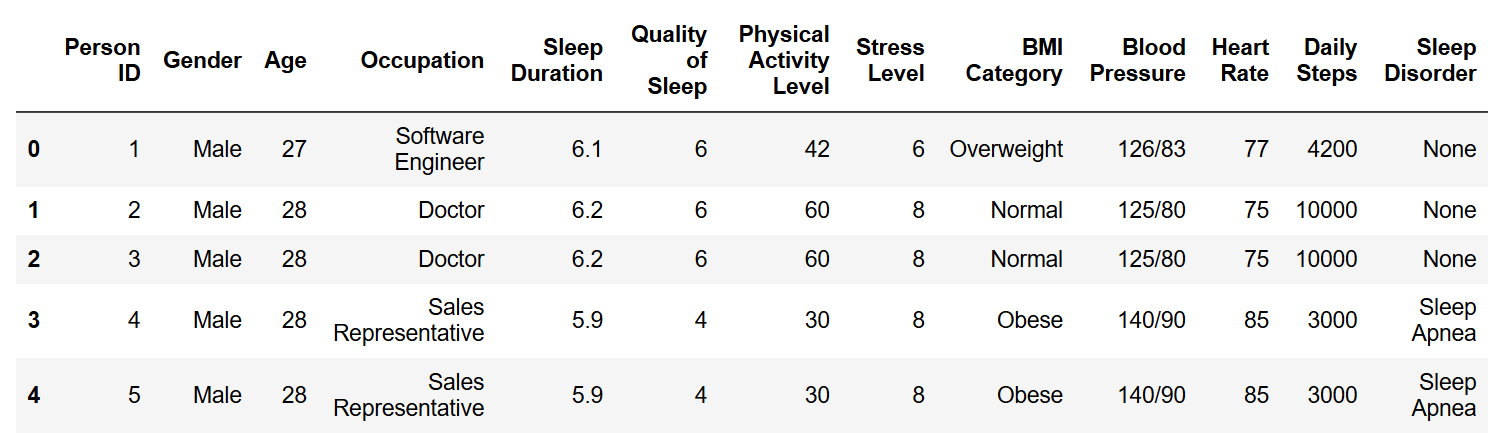
\includegraphics[width=1\linewidth]{img/datasetInicial.png}
    \caption{Dataset inicial.}
    \label{fig:dataset-inicial}
\end{figure}

A continuación se llevó a cabo una revisión estructural del dataset, aplicando distintos métodos de inspección:


\begin{itemize}
    \item \textbf{Tipos de datos:} se utilizó el método \texttt{df.info()} para verificar los tipos de datos de cada columna. Se identificaron 13 columnas: 8 numéricas y 5 categóricas (tipo \texttt{object}).

    \begin{figure}[H]
        \centering
        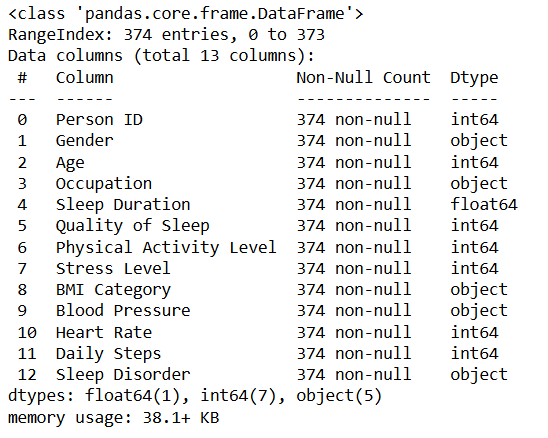
\includegraphics[width=0.75\linewidth]{img/df_info.png}
        \caption{Descripción de los tipos de datos de las variables del dataset.}
        \label{fig:df_info}
    \end{figure}
    
    \item \textbf{Valores nulos:} no se detectaron valores ausentes en ninguna columna (\texttt{df.isnull().sum()} devolvió cero en todos los casos), por lo que no fue necesario aplicar imputaciones.
    
    \item \textbf{Duplicados:} tampoco se encontraron registros duplicados (\texttt{df.duplicated().sum()} = 0), lo cual garantiza que cada fila representa a un individuo único.
    
    \item \textbf{Resumen estadístico:} el método \texttt{df.describe()} mostró que las variables numéricas presentaban rangos clínicamente válidos. Por ejemplo, la edad oscilaba entre 27 y 59 años, la frecuencia cardíaca entre 65 y 86 lpm, y la duración del sueño entre 5.8 y 8.5 horas.
    
    \begin{figure}[H]
        \centering
        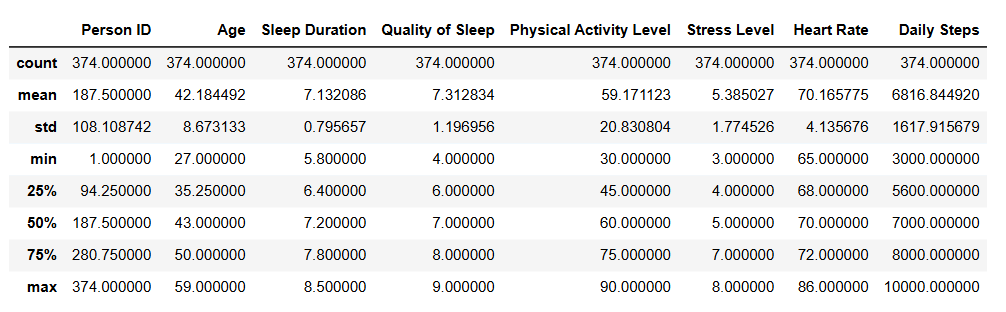
\includegraphics[width=0.9\linewidth]{img/df_describe.png}
        \caption{Resumen estadístico de las variables numéricas del dataset.}
        \label{fig:df_describe}
    \end{figure}
    
    \item \textbf{Variables categóricas:} se inspeccionaron los valores únicos de columnas como \texttt{Gender}, \texttt{Occupation} y \texttt{BMI Category}. Se identificaron dos categorías de género, once ocupaciones distintas y cuatro categorías de IMC (Índice de Masa Corporal). Se detectó una etiqueta duplicada en la variable \texttt{BMI Category} (“Normal Weight”), que se unificó con “Normal” para evitar ambigüedades durante la codificación.

    \begin{figure}[H]
        \centering
        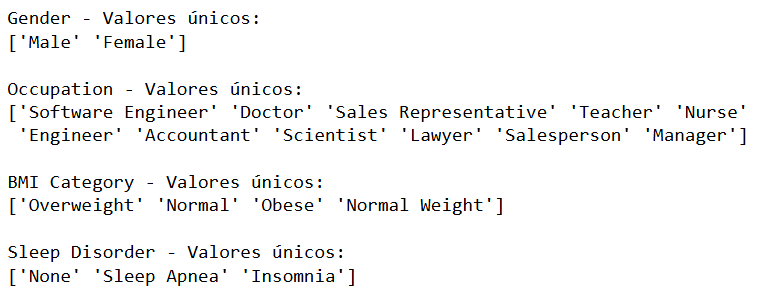
\includegraphics[width=0.8\linewidth]{img/columnasCategoricas.png}
        \caption{Descripción de los valores posibles en las variables categóricas.}
        \label{fig:columnas-categoricas}
    \end{figure}
    
\end{itemize}

\subsubsection{Eliminación de variables no predictivas}

Se eliminó la columna \texttt{Person ID}, ya que su única función era actuar como identificador único de registros. Al no aportar información útil para la predicción, se consideró una variable irrelevante desde el punto de vista del modelado.



\subsection{Análisis exploratorio de datos (EDA)}

El análisis exploratorio de datos (EDA, por sus siglas en inglés) constituye una etapa clave para comprender la estructura del conjunto de datos, identificar anomalías, explorar distribuciones y relaciones entre variables, y orientar las decisiones posteriores sobre preprocesamiento, selección de variables y diseño del modelo.


\subsubsection{Distribución de variables numéricas}

Para cada variable continua se generaron cuatro representaciones gráficas: \textbf{boxplot}, \textbf{violin plot}, \textbf{KDE plot} y \textbf{histograma}, con el objetivo de examinar su distribución, simetría y posibles valores atípicos desde distintos enfoques. A continuación, se muestran algunos ejemplos representativos.

\begin{figure}[H]
    \centering
    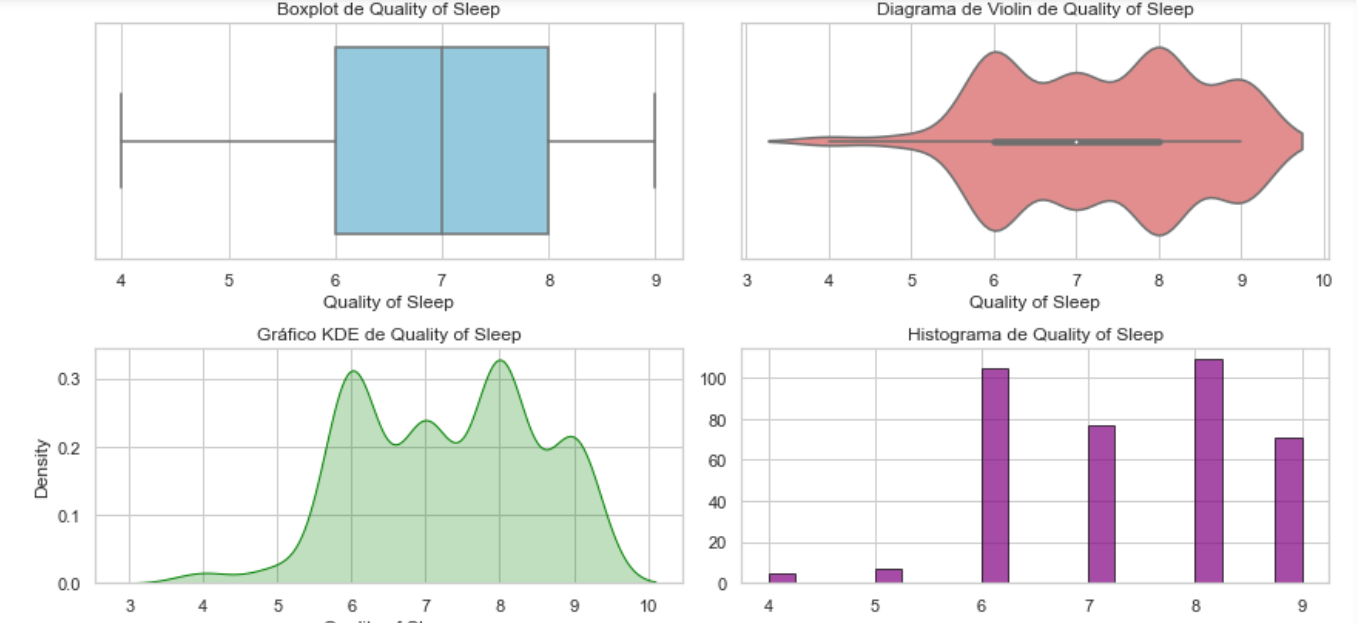
\includegraphics[width=1\linewidth]{img/qualitySleep.png}
    \caption{Distribución de la variable \textit{Quality of Sleep} mediante diferentes representaciones gráficas.}
\end{figure}

También se analizaron estas variables diferenciando por clase de trastorno del sueño, lo que permitió identificar patrones relevantes. Por ejemplo, se observó que los sujetos con insomnio tendían a concentrarse en valores bajos de duración del sueño.

\begin{figure}[H]
    \centering
    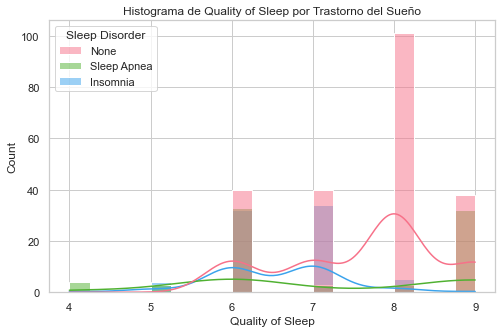
\includegraphics[width=1\linewidth]{img/qualityTrastorno.png}
    \caption{Distribución de la variable \textit{Quality of Sleep} por clase de trastorno del sueño mediante histograma con curva KDE.}
    \label{fig:hist_quality_sleep}
\end{figure}

\begin{figure}[H]
    \centering
    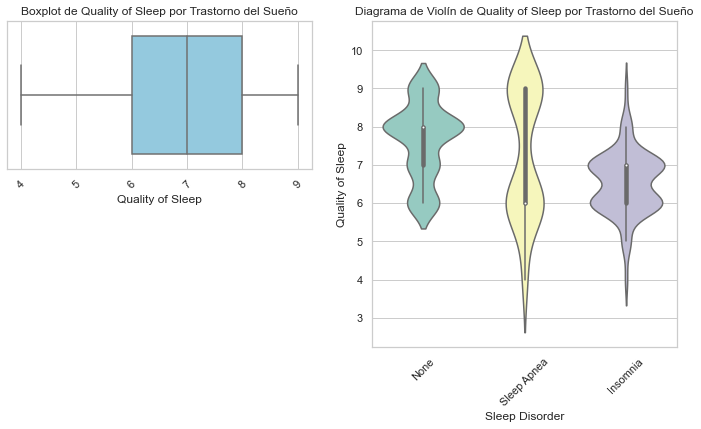
\includegraphics[width=1\linewidth]{img/qualityBoxTrastorno.png}
    \caption{Distribución de la variable \textit{Quality of Sleep} por clase de trastorno del sueño mediante boxplot y diagrama de violín.}
    \label{fig:box_violin_quality_sleep}
\end{figure}



\subsubsection{Distribución de variables categóricas}

Se exploraron visualmente las variables categóricas \texttt{Gender}, \texttt{Occupation}, \texttt{BMI Category} y \texttt{Sleep Disorder}. En la Figura~\ref{fig:ocupacion_clase}, se muestra la distribución de ocupaciones por clase.

\begin{figure}[H]
    \centering
    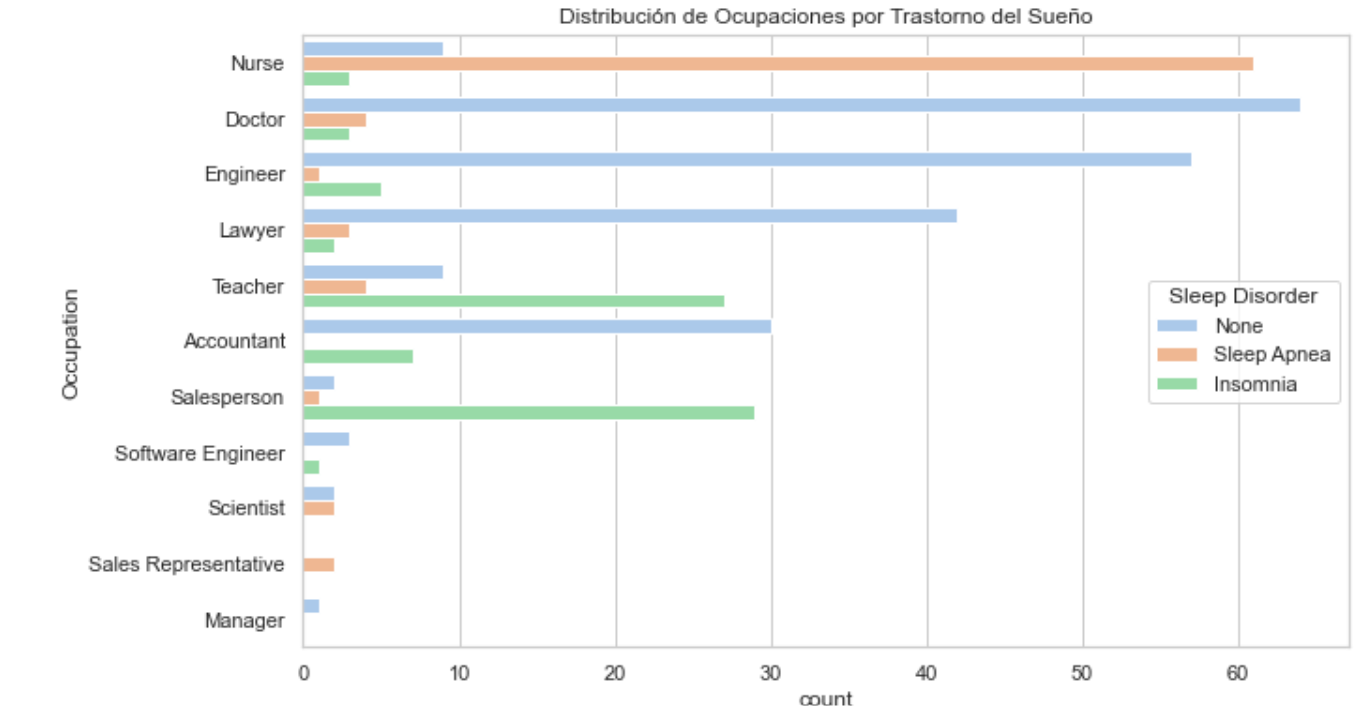
\includegraphics[width=1\linewidth]{img/ocupacionesClase.png}
    \caption{Distribución de la variable \texttt{Occupation} por clase.}
    \label{fig:ocupacion_clase}
\end{figure}

En la Figura~\ref{fig:bmi_trastorno} se muestra un ejemplo representativo, donde se observa que la categoría \textit{Normal} es predominante entre individuos sin trastorno, mientras que las categorías \textit{Overweight} y \textit{Obese} presentan mayor proporción de casos con apnea del sueño o insomnio.


\begin{figure}[H]
    \centering
    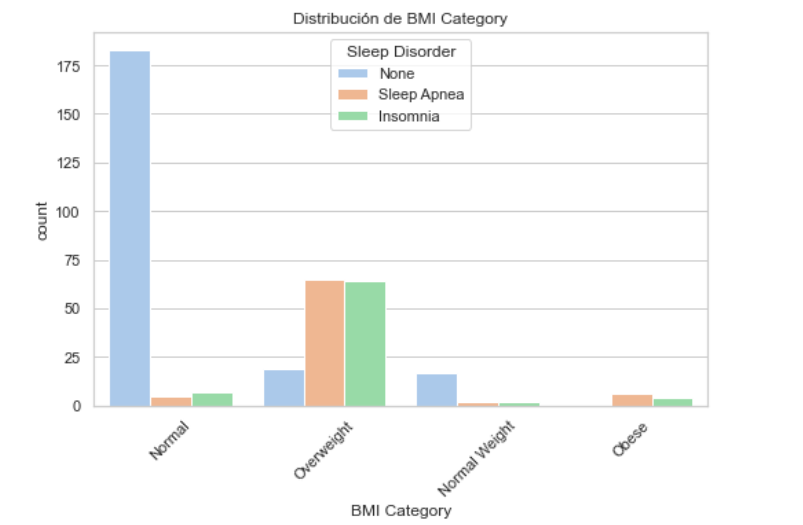
\includegraphics[width=1\linewidth]{img/IMCtrastorno.png}
    \caption{Distribución de categorías de IMC (\texttt{BMI Category}) según tipo de trastorno del sueño.}
    \label{fig:bmi_trastorno}
\end{figure}

Este análisis permitió observar que ciertas ocupaciones como \textit{Nurse} o \textit{Salesperson} estaban sobrerrepresentadas en casos de insomnio o apnea del sueño, lo que podría estar relacionado con patrones ocupacionales de riesgo, aportando una posible interpretación clínica.

\subsubsection{Detección de outliers}

Para complementar el análisis visual mediante diagramas de caja y violín, se aplicó un enfoque estadístico basado en el rango intercuartílico (IQR) con el objetivo de identificar valores atípicos de forma cuantitativa. Este método establece umbrales inferior y superior para cada variable numérica, definidos como:

\[
\text{IQR} = Q_3 - Q_1 \qquad 
\text{Límite inferior} = Q_1 - 1.5 \cdot \text{IQR} \qquad 
\text{Límite superior} = Q_3 + 1.5 \cdot \text{IQR}
\]

Se evaluaron las siguientes variables numéricas: edad, duración del sueño, calidad del sueño, nivel de estrés, pasos diarios, frecuencia cardíaca y nivel de actividad física. Como resultado, se identificaron un total de 15 registros con valores fuera de los límites definidos, todos ellos correspondientes a la variable \texttt{Heart Rate}.


\begin{table}[H]
    \centering
    \begin{tabular}{l|c}
        \textbf{Variable} & \textbf{Outliers detectados} \\
        \hline
        Heart Rate & 15 \\
        Todas las demás & 0
    \end{tabular}
    \caption{Número de outliers detectados por variable (método IQR).}
\end{table}

Estos registros no fueron eliminados del conjunto de datos, ya que se consideró que podrían representar condiciones clínicas reales, como bradicardia, que pueden ser relevantes para el diagnóstico de ciertos trastornos del sueño. Esta decisión se tomó en línea con el criterio clínico de conservar la heterogeneidad natural de la muestra.



\subsubsection{Correlaciones entre variables}

Se construyó un mapa de calor con el coeficiente de correlación de Pearson para identificar relaciones lineales entre variables numéricas. Destacó una fuerte correlación positiva entre presión sistólica y diastólica ($r \approx 0.97$), así como una correlación negativa entre calidad del sueño y nivel de estrés.

\begin{figure}[H]
    \centering
    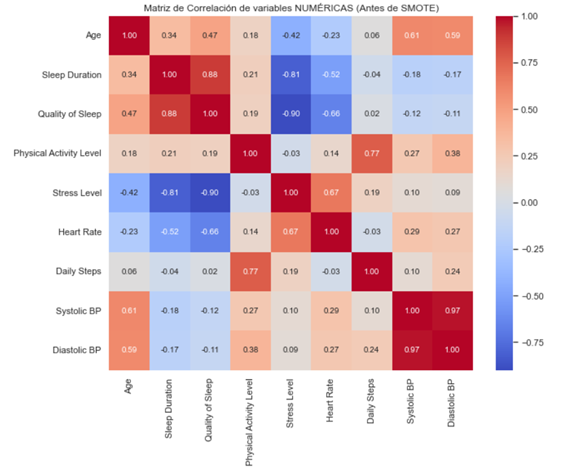
\includegraphics[width=1\linewidth]{img/heatmap.png}
    \caption{Mapa de correlaciones entre variables numéricas.}
    \label{fig:heatmap}
\end{figure}

\subsubsection{Distribución de la variable objetivo}

La variable objetivo \texttt{Sleep Disorder} incluye tres clases: \texttt{None}, \texttt{Insomnia} y \texttt{Sleep Apnea}. En la Figura~\ref{fig:dist_clases} se observa un claro desbalance: la clase \texttt{None} representa más del 50\% de los registros, mientras que las clases patológicas tienen una representación significativamente menor.

\begin{figure}[H]
    \centering
    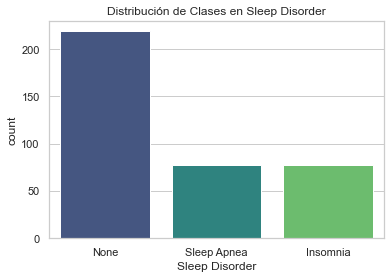
\includegraphics[width=0.75\linewidth]{img/countplot_SleepDisorders.png}
    \caption{Distribución de clases en la variable \textit{Sleep Disorder}.}
    \label{fig:dist_clases}
\end{figure}

Este desequilibrio fue tenido en cuenta durante la fase de modelado, donde se evaluaron técnicas de balanceo específicas que se describen más adelante.


\subsubsection{Importancia de características}

Como parte del análisis exploratorio, se evaluó la influencia relativa de cada variable sobre la predicción de los trastornos del sueño. Se aplicaron múltiples técnicas de selección de características, tanto basadas en modelos como en estadística:

\begin{itemize}
    \item \textbf{Random Forest:} se analizaron las reducciones de impureza en cada nodo para estimar la importancia de las variables. La Figura~\ref{fig:feature_rf} muestra el resultado de este análisis.
    \item \textbf{SelectKBest:} se utilizaron pruebas estadísticas como $\chi^2$ (para variables categóricas) y ANOVA-F (para numéricas) para valorar la relación con la variable objetivo.
    \item \textbf{RFE (Recursive Feature Elimination):} se entrenó un modelo de regresión logística que eliminaba iterativamente las variables menos relevantes hasta seleccionar las más influyentes.
\end{itemize}

\begin{figure}[H]
    \centering
    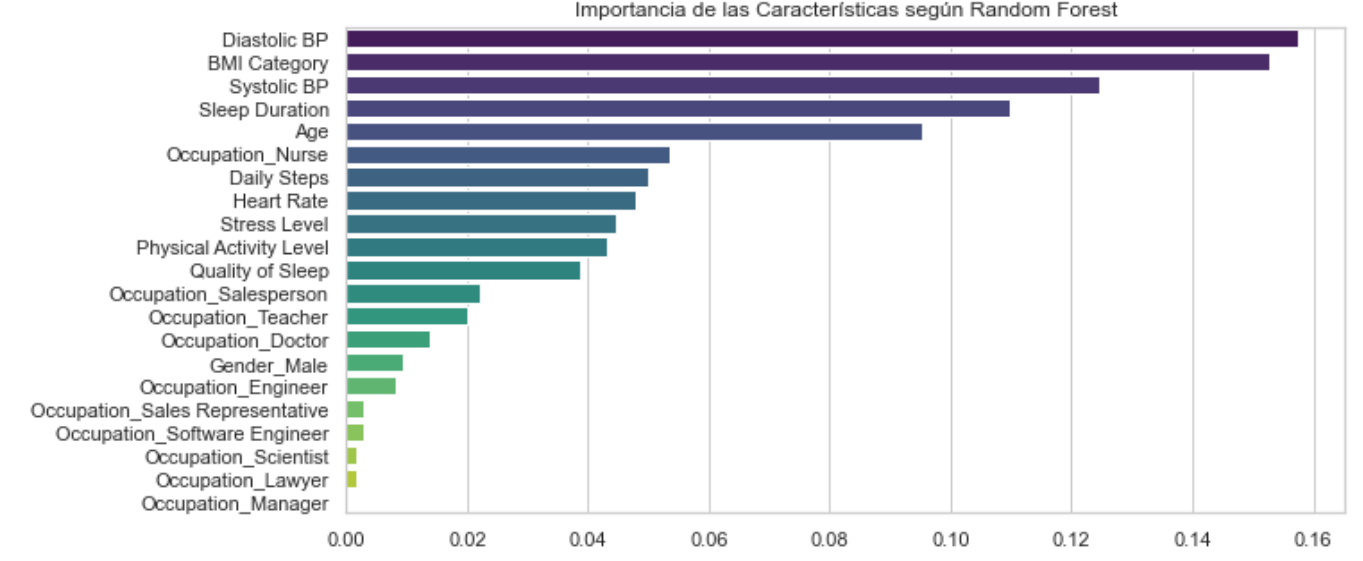
\includegraphics[width=1\linewidth]{img/importanciaRF.png}
    \caption{Importancia de características según Random Forest.}
    \label{fig:feature_rf}
\end{figure}

Las variables más destacadas por varias técnicas fueron: \textit{BMI Category}, \textit{Diastolic BP}, \textit{Occupation\_Nurse} y \textit{Sleep Duration}. No obstante, se optó por conservar todas las variables, priorizando la interpretabilidad y evitando eliminar características que podrían tener valor clínico no capturado por su peso estadístico.


El análisis exploratorio no solo permitió detectar posibles sesgos en la distribución de las clases y evaluar la calidad general del dataset, sino también orientar decisiones clave en el diseño del modelo, como la necesidad de calibración, la selección de variables relevantes y la elección de algoritmos robustos frente al desbalance de clases. 

Este análisis estableció así una base sólida para el posterior preprocesamiento de los datos, asegurando que las transformaciones aplicadas respondieran a patrones reales del conjunto y no a artefactos o desequilibrios ocultos.



\subsection{Preprocesamiento}

Una vez finalizado el análisis exploratorio, se procedió al preprocesamiento del conjunto de datos. Esta fase incluyó transformaciones esenciales para preparar las variables para su uso eficiente en modelos de aprendizaje automático, garantizando al mismo tiempo la coherencia clínica y semántica de la información.


\subsubsection{Codificación de variables categóricas}

Las variables categóricas se transformaron en variables numéricas utilizando dos enfoques diferenciados:

\begin{itemize}
    \item \textbf{One-Hot Encoding}, aplicado a variables nominales como \texttt{Gender} y \texttt{Occupation}, generando una columna binaria por cada categoría posible.
    \item \textbf{Label Encoding}, utilizado para la variable ordinal \texttt{BMI Category}, respetando su orden lógico clínico: \textit{Underweight < Normal < Overweight < Obese}.
\end{itemize}

El uso combinado de codificación binaria para variables nominales y ordinal para escalas clínicas asegura que la semántica original no se pierda durante el modelado. Tras la codificación, se conservaron todas las variables generadas, incluyendo las columnas binarias del \textit{one-hot encoding}, con el objetivo de mantener el máximo contexto clínico durante la predicción.

\subsubsection{Estandarización de variables numéricas}

Con el fin de homogeneizar la escala de las variables continuas y facilitar su procesamiento por parte de los algoritmos, se aplicaron técnicas de escalado a las siguientes variables:

\begin{itemize}
    \item Age
    \item Sleep Duration
    \item Quality of Sleep
    \item Physical Activity Level
    \item Stress Level
    \item Daily Steps
    \item Heart Rate
    \item Systolic BP
    \item Diastolic BP
\end{itemize}

Aunque inicialmente se evaluó el uso de \texttt{StandardScaler}, que transforma los datos a una distribución con media cero y desviación estándar uno, se observó que este método generaba valores negativos, lo cual dificultaba la representación visual en la aplicación interactiva y reducía su interpretabilidad para usuarios no técnicos. Por ello, se optó finalmente por \texttt{MinMaxScaler}, que transforma las variables al rango [0, 1], preservando la proporcionalidad relativa entre valores y facilitando su uso clínico y visual.


\subsubsection{División del conjunto de datos}

Finalmente, se realizó la partición del dataset en dos subconjuntos: un 80\% para entrenamiento y un 20\% para validación. Se utilizó la función \texttt{train\_test\_split} con la opción de \textbf{estratificación} sobre la variable \texttt{Sleep Disorder}, asegurando así que la distribución de clases se mantuviera proporcional en ambos subconjuntos. Esta estrategia es especialmente importante en tareas multiclase con clases desbalanceadas, como en este caso, donde la clase \texttt{None} es mayoritaria.

Tras completar estas transformaciones, el conjunto de datos quedó preparado para su uso en las fases de entrenamiento, validación cruzada y evaluación comparativa de modelos multiclase.


\begin{table}[H]
\centering
\begin{tabular}{ll}
\toprule
\textbf{Proceso} & \textbf{Descripción} \\
\midrule
Codificación      & One-Hot y Label Encoding \\
Escalado          & MinMaxScaler (rango [0, 1]) \\
Partición de datos & 80\% entrenamiento / 20\% test, con estratificación \\
\bottomrule
\end{tabular}
\caption{Resumen de las transformaciones aplicadas durante el preprocesamiento.}
\end{table}


\subsection{Desarrollo y selección de modelos predictivos}

Una vez completado el preprocesamiento, se procedió al entrenamiento de distintos modelos de clasificación multiclase con el objetivo de predecir si un individuo presenta insomnio, apnea del sueño o ausencia de trastornos. Para ello, se evaluaron cinco algoritmos clásicos de aprendizaje automático, implementados en la biblioteca \textit{scikit-learn}\footnote{\href{https://scikit-learn.org/}{Librería de scikit-learn.}}:

\begin{itemize}
    \item Regresión logística (\textit{Logistic Regression})
    \item Árboles de decisión (\textit{Decision Tree})
    \item Máquina de vectores soporte (\textit{SVM})
    \item Perceptrón multicapa (\textit{MLP})
    \item Bosques aleatorios (\textit{Random Forest})
\end{itemize}

La evaluación inicial se realizó mediante validación cruzada estratificada (\texttt{StratifiedKFold}) con cinco particiones (k=5). Como métrica principal se utilizó el \textbf{F1-score macro}, al ofrecer un mejor equilibrio entre clases desbalanceadas y evitar que la clase mayoritaria dominara el análisis global.

\subsubsection{Comparación inicial y efecto de SMOTE}

Dado el desequilibrio en la distribución de clases (mostrado en la Figura \ref{fig:dist_clases}) del conjunto de entrenamiento (\textit{None}: 175, \textit{Sleep Apnea}: 62, \textit{Insomnia}: 62), se evaluó la viabilidad de aplicar la técnica de sobremuestreo \textbf{SMOTE} (Synthetic Minority Oversampling Technique). Esta técnica genera ejemplos sintéticos de las clases minoritarias a partir de combinaciones lineales de muestras reales y sus vecinos más cercanos.

SMOTE se aplicó exclusivamente sobre el conjunto de entrenamiento, evitando así fugas de información. La distribución equilibrada resultante se muestra en la Figura~\ref{fig:distribucion_smote}.


\begin{figure}[H]
    \centering
    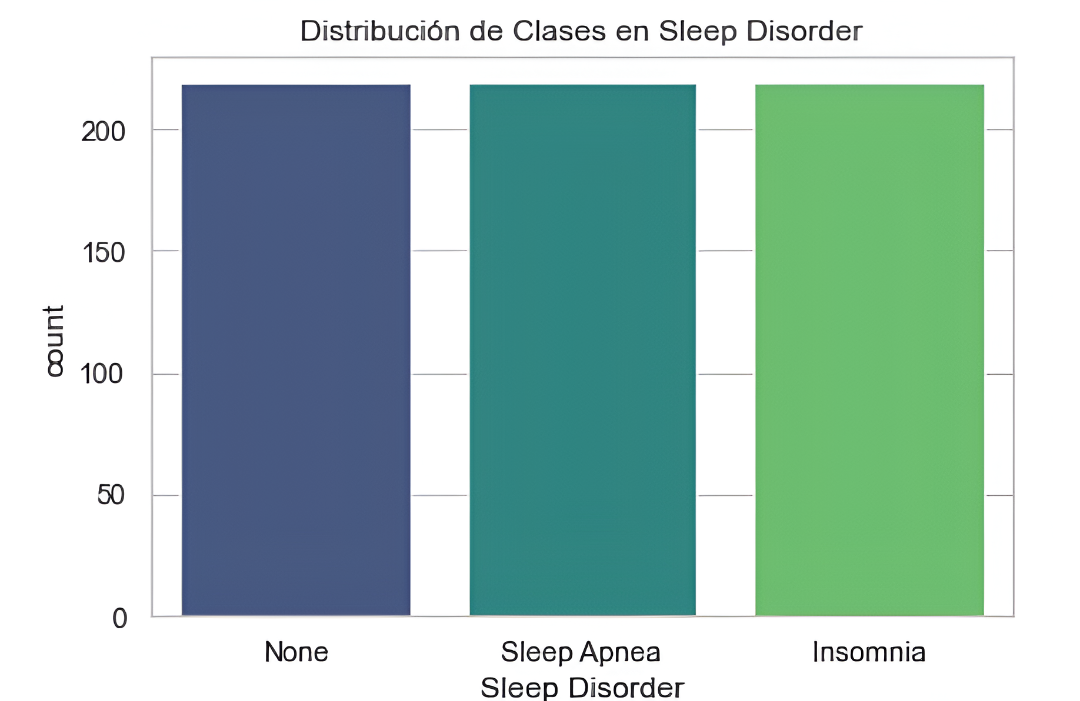
\includegraphics[width=0.75\linewidth]{img/sleepDesorder_smote.png}
    \caption{Distribución de clases tras aplicar SMOTE en el conjunto de entrenamiento.}
    \label{fig:distribucion_smote}
\end{figure}

Los resultados obtenidos con esta técnica se presentan y analizan en el capítulo de \ref{cap:resultados} Resultados.


\subsubsection{Ajuste de hiperparámetros}

Para cada modelo se llevó a cabo una fase de ajuste de hiperparámetros utilizando \texttt{RandomizedSearchCV} o \texttt{GridSearchCV}, en función del espacio de búsqueda y la complejidad computacional. En todos los casos se aplicó validación cruzada estratificada (k=5) sobre el conjunto de entrenamiento y se seleccionó el estimador que maximizaba el F1-score macro.

Los hiperparámetros explorados fueron:

\begin{itemize}
    \item \textbf{Random Forest:} \verb|n_estimators|, \verb|max_depth|, \verb|min_samples_split|, \verb|min_samples_leaf|, \verb|bootstrap|.
    \item \textbf{MLP:} \verb|hidden_layer_sizes|, \verb|activation|, \verb|solver|, \verb|alpha|, \verb|learning_rate|.
    \item \textbf{Regresión Logística:} \verb|penalty|, \verb|C|, \verb|solver|.
    \item \textbf{Decision Tree:} \verb|max_depth|, \verb|min_samples_leaf|, \verb|min_samples_split|, \verb|criterion|.
    \item \textbf{SVM:} \verb|C|, \verb|kernel|, \verb|gamma|.
\end{itemize}

Cada modelo óptimo fue almacenado para su posterior calibración, evaluación comparativa y posible integración en la aplicación web.

%%%% conceptos teoricos 3.6
\subsubsection{Criterios de evaluación clínica del modelo}

En el presente trabajo se abordó un problema de clasificación multiclase, cuyo objetivo era asignar a cada individuo una de tres clases posibles: \textit{None}, \textit{Insomnia} o \textit{Sleep Apnea}. La naturaleza desbalanceada de estas clases, así como la relevancia clínica de los falsos negativos y falsos positivos, exigió una evaluación más detallada que la mera tasa de aciertos.

\textbf{Matriz de confusión}\\

La matriz de confusión permite comparar las predicciones del modelo con las etiquetas reales, descomponiendo el rendimiento en los siguientes componentes:

\begin{itemize}
    \item \textbf{True Positives (TP)}: casos positivos correctamente clasificados.
    \item \textbf{True Negatives (TN)}: casos negativos correctamente clasificados.
    \item \textbf{False Positives (FP)}: casos negativos clasificados erróneamente como positivos.
    \item \textbf{False Negatives (FN)}: casos positivos que el modelo no ha detectado.
\end{itemize}

\textbf{Métricas derivadas}\\

A partir de esta matriz se calcularon las siguientes métricas:

\begin{itemize}
    \item \textbf{Accuracy} (exactitud): proporción total de aciertos del modelo.
    \begin{equation}
        \text { Accuracy }=\frac{TP+TN}{TP+TN+FP+FN}
    \end{equation}
    Aunque es una métrica útil como referencia general, puede ser engañosa en conjuntos desbalanceados.

    \item \textbf{Precision}: porcentaje de predicciones positivas que realmente lo son.
    \begin{equation}
        \text { Precision }=\frac{TP}{TP+FP}
    \end{equation}
    Esta métrica ayuda a controlar los falsos positivos, clave en contextos clínicos sensibles.

    \item \textbf{Recall} (sensibilidad):
    \begin{equation}
        \text { Recall }=\frac{TP}{TP + FN}
    \end{equation}
    Es crítica cuando el objetivo es no dejar casos sin detectar, como en el diagnóstico de apnea o insomnio.

    \item \textbf{F1-score}:
    \begin{equation}
        F1 = 2 \cdot \frac{\text { Precision } \cdot \text { Recall }}  {\text { Precision }+ \text { Recall }}
    \end{equation}
    Se trata de la media armónica entre precisión y recall, recomendada en contextos con clases poco representadas.

\end{itemize}

En este trabajo se utilizó el \textbf{F1-score macro}, que calcula el F1-score de cada clase por separado y luego hace la media no ponderada. Esto evita que la clase mayoritaria domine el análisis.

\textbf{Evaluación gráfica}\\

Para complementar las métricas numéricas, se utilizaron dos representaciones gráficas adicionales:

\begin{itemize}
    \item \textbf{Curva ROC-AUC (Receiver Operating Characteristic)}: muestra la relación entre la tasa de verdaderos positivos (TP) y la tasa de falsos positivos (FP) para distintos umbrales de decisión. El área bajo esta curva (AUC) resume la capacidad discriminativa del modelo:
    \begin{itemize}
        \item AUC = 0.5: rendimiento equivalente al azar.
        \item AUC = 1.0: modelo perfecto.
    \end{itemize}

    \item \textbf{Curva Precision-Recall (PR)}: especialmente útil en contextos clínicos desbalanceados. Representa el compromiso entre precisión y recall a diferentes umbrales, proporcionando una visión más realista de la eficacia del modelo en las clases minoritarias.
\end{itemize}

El uso conjunto de estas métricas permitió evaluar de manera robusta la calidad del modelo tanto a nivel global como por clase. Los valores obtenidos y sus implicaciones se analizan en el capítulo de \textbf{Resultados} (\ref{cap:resultados}) \cite{powers2020evaluation}.


\subsubsection{Análisis de la influencia de la variable \texttt{Occupation}}

Durante el análisis exploratorio se detectó que la variable \texttt{Occupation}, codificada mediante \textit{One-Hot Encoding}, mostraba asociaciones notables con las clases patológicas, especialmente con insomnio y apnea del sueño. Esta observación planteó la hipótesis de que el modelo pudier estar capturando patrones no generalizables derivados del pequeño tamaño del conjunto de datos o de correlaciones espurias.

Con el fin de valorar el impacto específico de esta variable, se desarrolló una versión alternativa del pipeline completo de entrenamiento en la que \texttt{Occupation} fue excluida antes del preprocesamiento. En esta variante se mantuvieron todas las transformaciones, técnicas de escalado, divisiones de datos y procedimientos de ajuste de hiperparámetros empleados en el modelo principal, de modo que la única diferencia fuera la presencia o ausencia de dicha variable.

Esta experimentación permitió establecer una base comparativa para evaluar en qué medida la variable ocupacional contribuía al rendimiento y comportamiento del sistema predictivo. Los resultados derivados de esta comparación se presentan y analizan en detalle en el capítulo~\ref{cap:resultados}.


\subsection{Interpretabilidad del modelo}

La interpretabilidad es especialmente relevante en el ámbito clínico, donde cada predicción automatizada puede influir en la toma de decisiones sobre la salud de una persona. Por ello, además de seleccionar el modelo \textit{Random Forest} como predeterminado por su rendimiento, se evaluó también su capacidad explicativa mediante técnicas de inteligencia artificial explicable.

El análisis de interpretabilidad se integró como parte del sistema para reforzar la confianza del usuario y garantizar que las decisiones del modelo puedan ser comprendidas tanto por profesionales como por pacientes.

\subsubsection{Importancia global de las variables}

Se generó un \textit{summary plot} (gráfico resumen) utilizando SHAP (\textit{SHapley Additive exPlanations}) para identificar las variables con mayor influencia en el conjunto de predicciones. Las características más relevantes fueron:

\begin{itemize}
    \item Presión arterial sistólica y diastólica
    \item Índice de masa corporal (BMI)
    \item Frecuencia cardíaca
    \item Duración del sueño
\end{itemize}

Las variables identificadas como más relevantes por SHAP coinciden con factores de riesgo ampliamente documentados en la literatura clínica, lo que refuerza la coherencia del modelo y su aceptación clínica.

\begin{figure}[H]
    \centering
    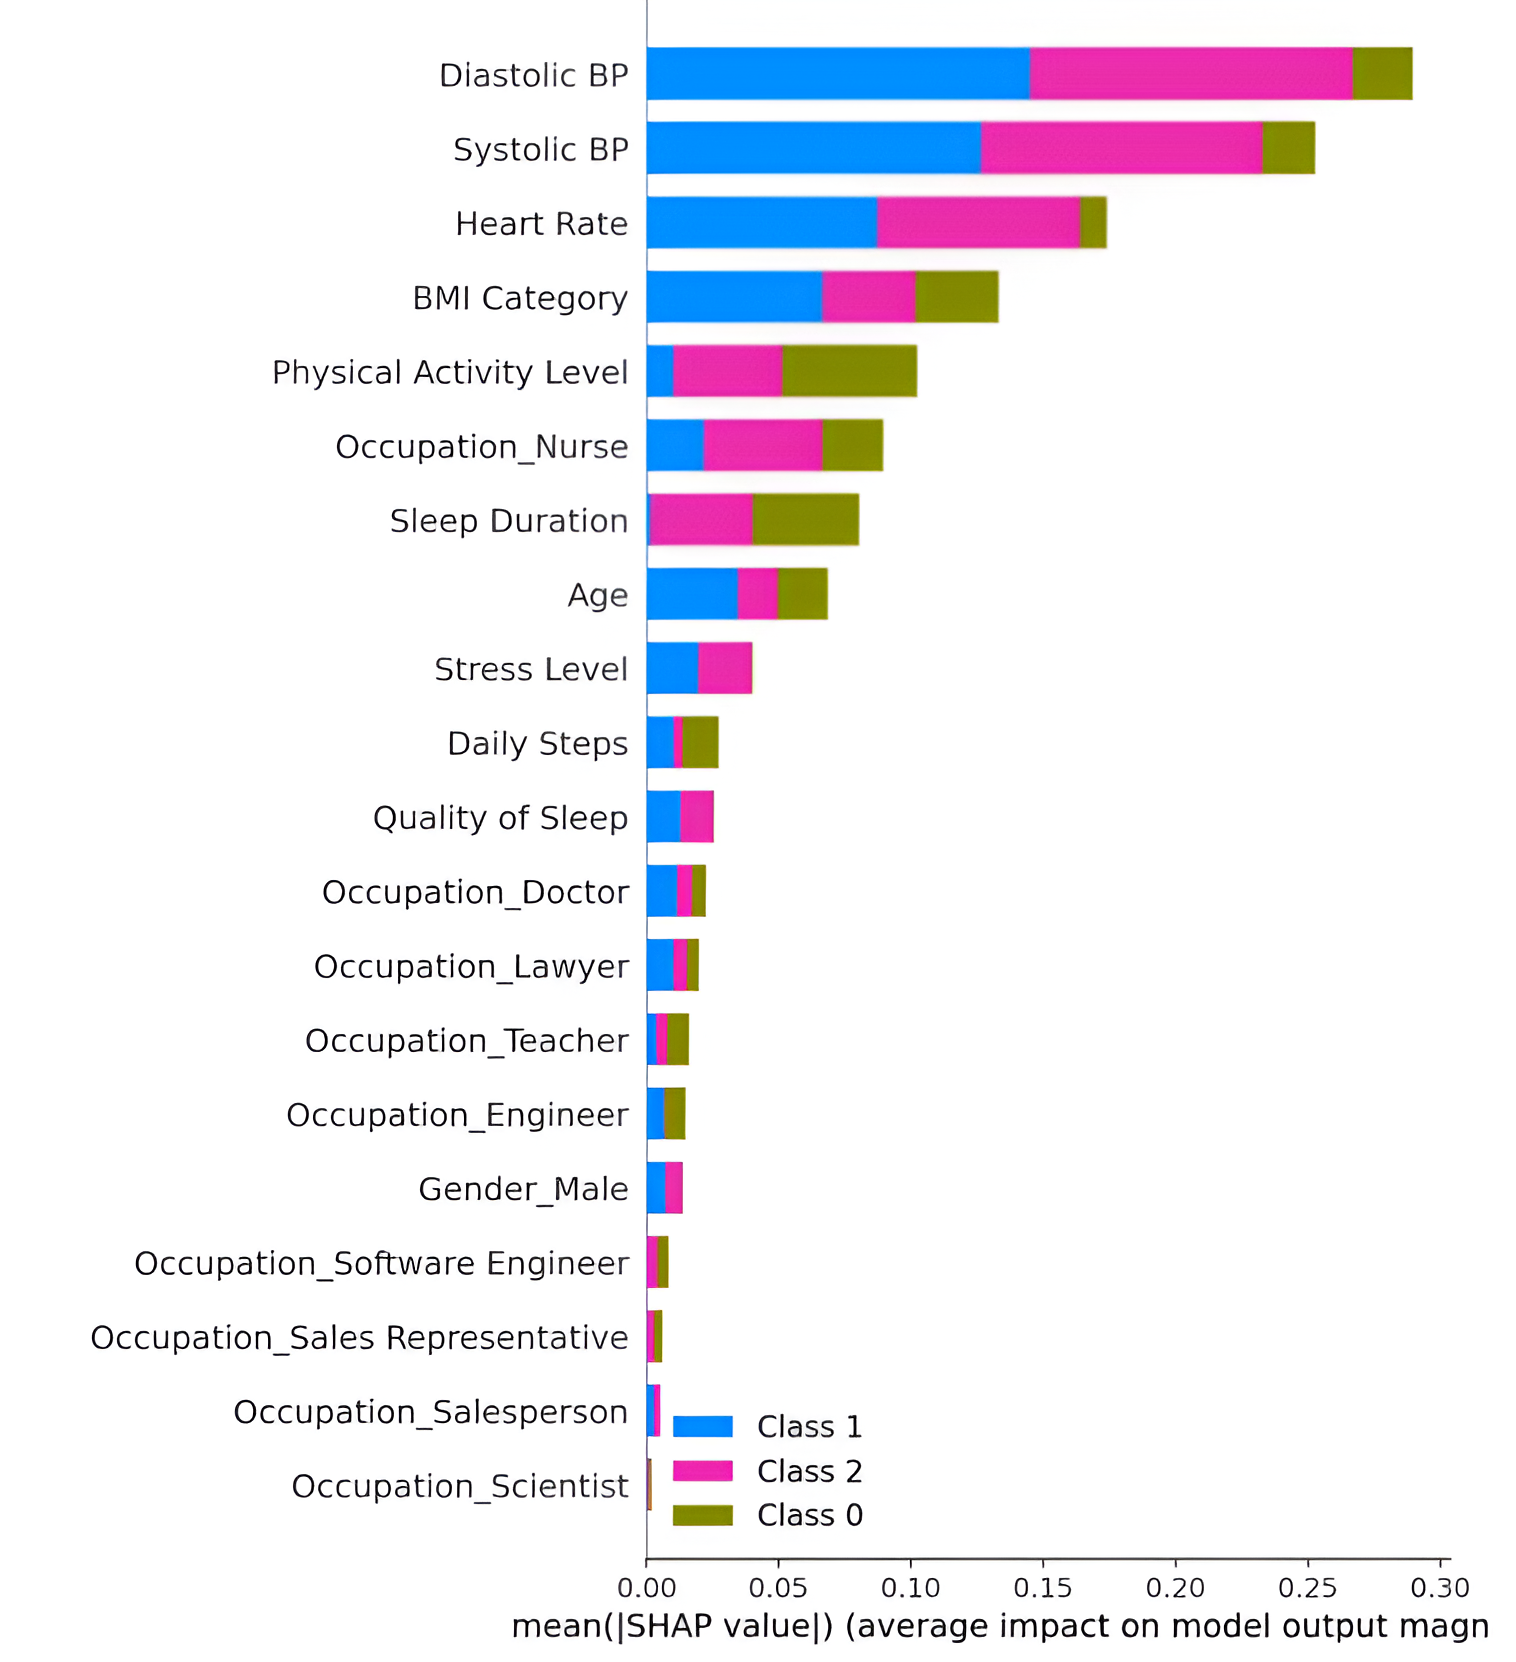
\includegraphics[width=0.85\linewidth]{img/SHAP.png}
    \caption{Gráfico resumen de SHAP: importancia media de cada variable}
    \label{fig:shap_summary}
\end{figure}

\subsubsection{Explicación individual de predicciones}
Para facilitar la interpretación de predicciones individuales, se utilizaron \textit{force plots} de SHAP. Estos gráficos descomponen la predicción mostrando cómo cada variable empuja la probabilidad hacia una clase concreta.

\begin{figure}[H]
    \centering
    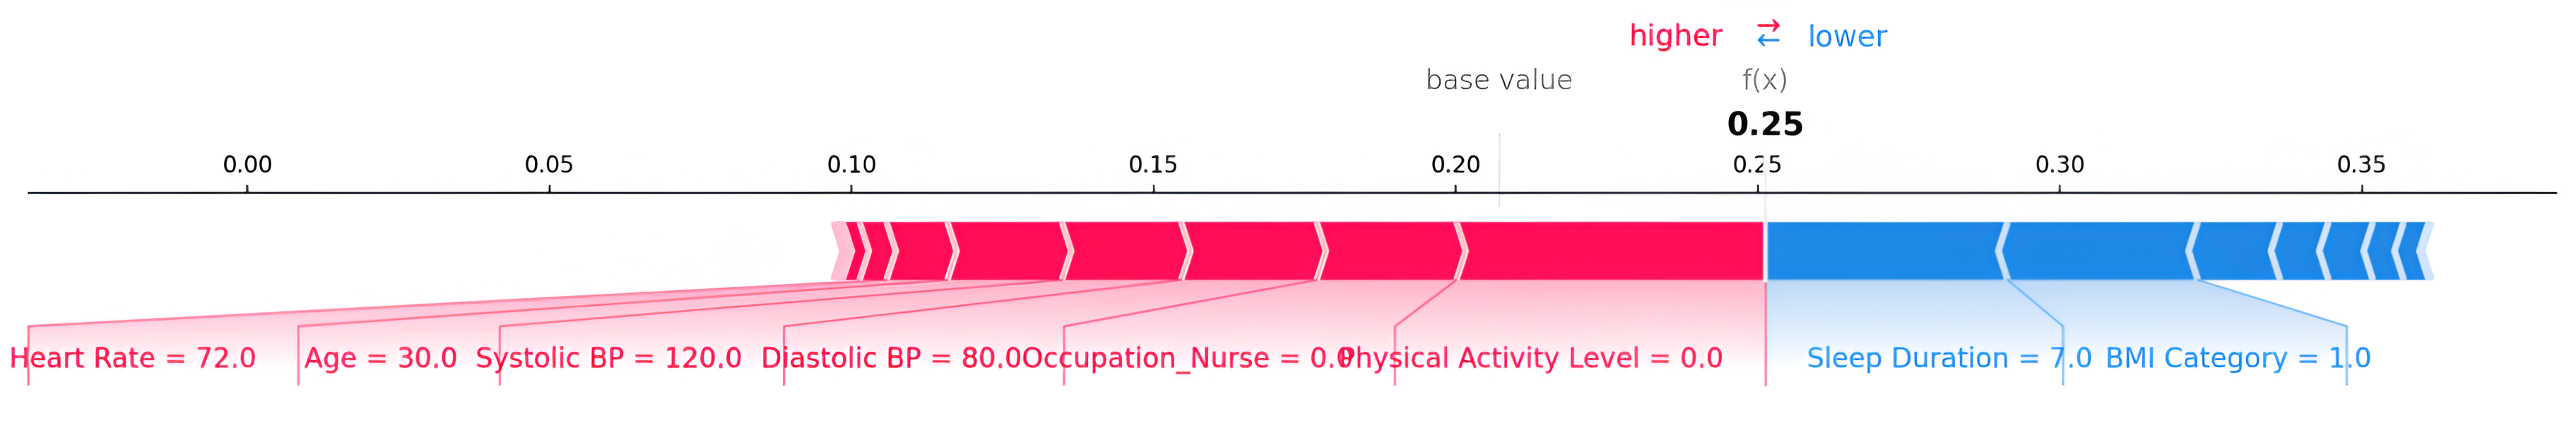
\includegraphics[width=1\linewidth]{img/explicacIndividual.png}
    \caption{Ejemplo de force plot para un individuo concreto}
    \label{fig:shap_force}
\end{figure}

Este enfoque mejora la transparencia del sistema y refuerza su utilidad en contextos donde se requiere trazabilidad de las decisiones.

\section{Implementación de la aplicación}

Con el objetivo de acercar el modelo predictivo al usuario final y facilitar su uso en contextos reales, se desarrolló una aplicación web interactiva mediante la librería \texttt{Streamlit}. Esta herramienta permitió construir una interfaz funcional directamente desde scripts de Python, sin necesidad de conocimientos en tecnologías web como HTML o JavaScript. El resultado fue una aplicación funcional, ligera y accesible desde cualquier dispositivo con conexión a internet.

\subsection{Objetivo y funcionalidades principales}

La aplicación permite introducir características personales y clínicas, realizar una predicción automática sobre el tipo de trastorno del sueño (o su ausencia), visualizar explicaciones basadas en SHAP y generar un informe en formato PDF.

El flujo de funcionamiento se estructura en las siguientes etapas:

\begin{enumerate}
    \item \textbf{Entrada de datos:} el usuario completa un formulario organizado en bloques, incluyendo edad, género, ocupación, calidad del sueño, presión arterial, IMC, nivel de estrés, pasos diarios, etc.
    \item \textbf{Preprocesamiento automático:} los datos son transformados mediante los mismos pasos aplicados en el entrenamiento (normalización y codificación One-Hot).
    \item \textbf{Predicción:} el modelo realiza la clasificación y devuelve las probabilidades asociadas a cada clase.
    \item \textbf{Visualización del resultado:} se muestra de forma clara la clase más probable junto con la probabilidad porcentual de cada una.
    \item \textbf{Explicabilidad:} se generan dos tipos de gráficos de SHAP: uno individual, que muestra qué variables influyeron más en la predicción concreta del usuario, y otro resumen global, que representa la importancia promedio de cada variable en el conjunto de datos.
    \item \textbf{Generación de informe:} se crea automáticamente un archivo PDF resumen con los datos introducidos, la predicción y la explicación visual.
\end{enumerate}

\subsection{Diseño y usabilidad}

La interfaz fue diseñada con criterios de claridad y usabilidad. Se utilizaron componentes interactivos como deslizadores, listas desplegables y botones de selección para facilitar la entrada de datos. El formulario está estructurado en dos columnas para una mejor experiencia visual, y los resultados se presentan con métricas porcentuales.

Además, se integraron funcionalidades adicionales como:

\begin{itemize}
    \item \textbf{Código QR dinámico:} insertado en la barra lateral para facilitar el acceso desde dispositivos móviles.
    \item \textbf{Generación automática de informes PDF:} utilizando la librería \texttt{FPDF}, con diseño clínico e información personalizada.
    \item \textbf{Gráficos SHAP:} tanto a nivel global (importancia de variables) como individual (force plot por paciente).
\end{itemize}

\subsection{Despliegue y validación}

La aplicación fue desplegada en la nube mediante \textbf{Streamlit Community Cloud}, lo que garantiza su accesibilidad sin necesidad de instalación local.

Para comprobar su correcto funcionamiento técnico, se realizaron pruebas de uso con distintos perfiles de entrada, simulando casos representativos de cada clase objetivo: sujetos sanos, con insomnio y con apnea del sueño. Estas pruebas permitieron validar el correcto flujo de datos desde el formulario hasta la generación de resultados e informes.

Adicionalmente, se contrastaron algunos perfiles simulados con informes reales obtenidos mediante el dispositivo O2Ring, durante una fase preliminar de desarrollo. Aunque no se realizó una integración directa con el dispositivo, esta comparación cualitativa permitió verificar la coherencia clínica del sistema y reforzar su aplicabilidad como herramienta complementaria de cribado o sensibilización.


\begin{figure}[H]
    \centering
    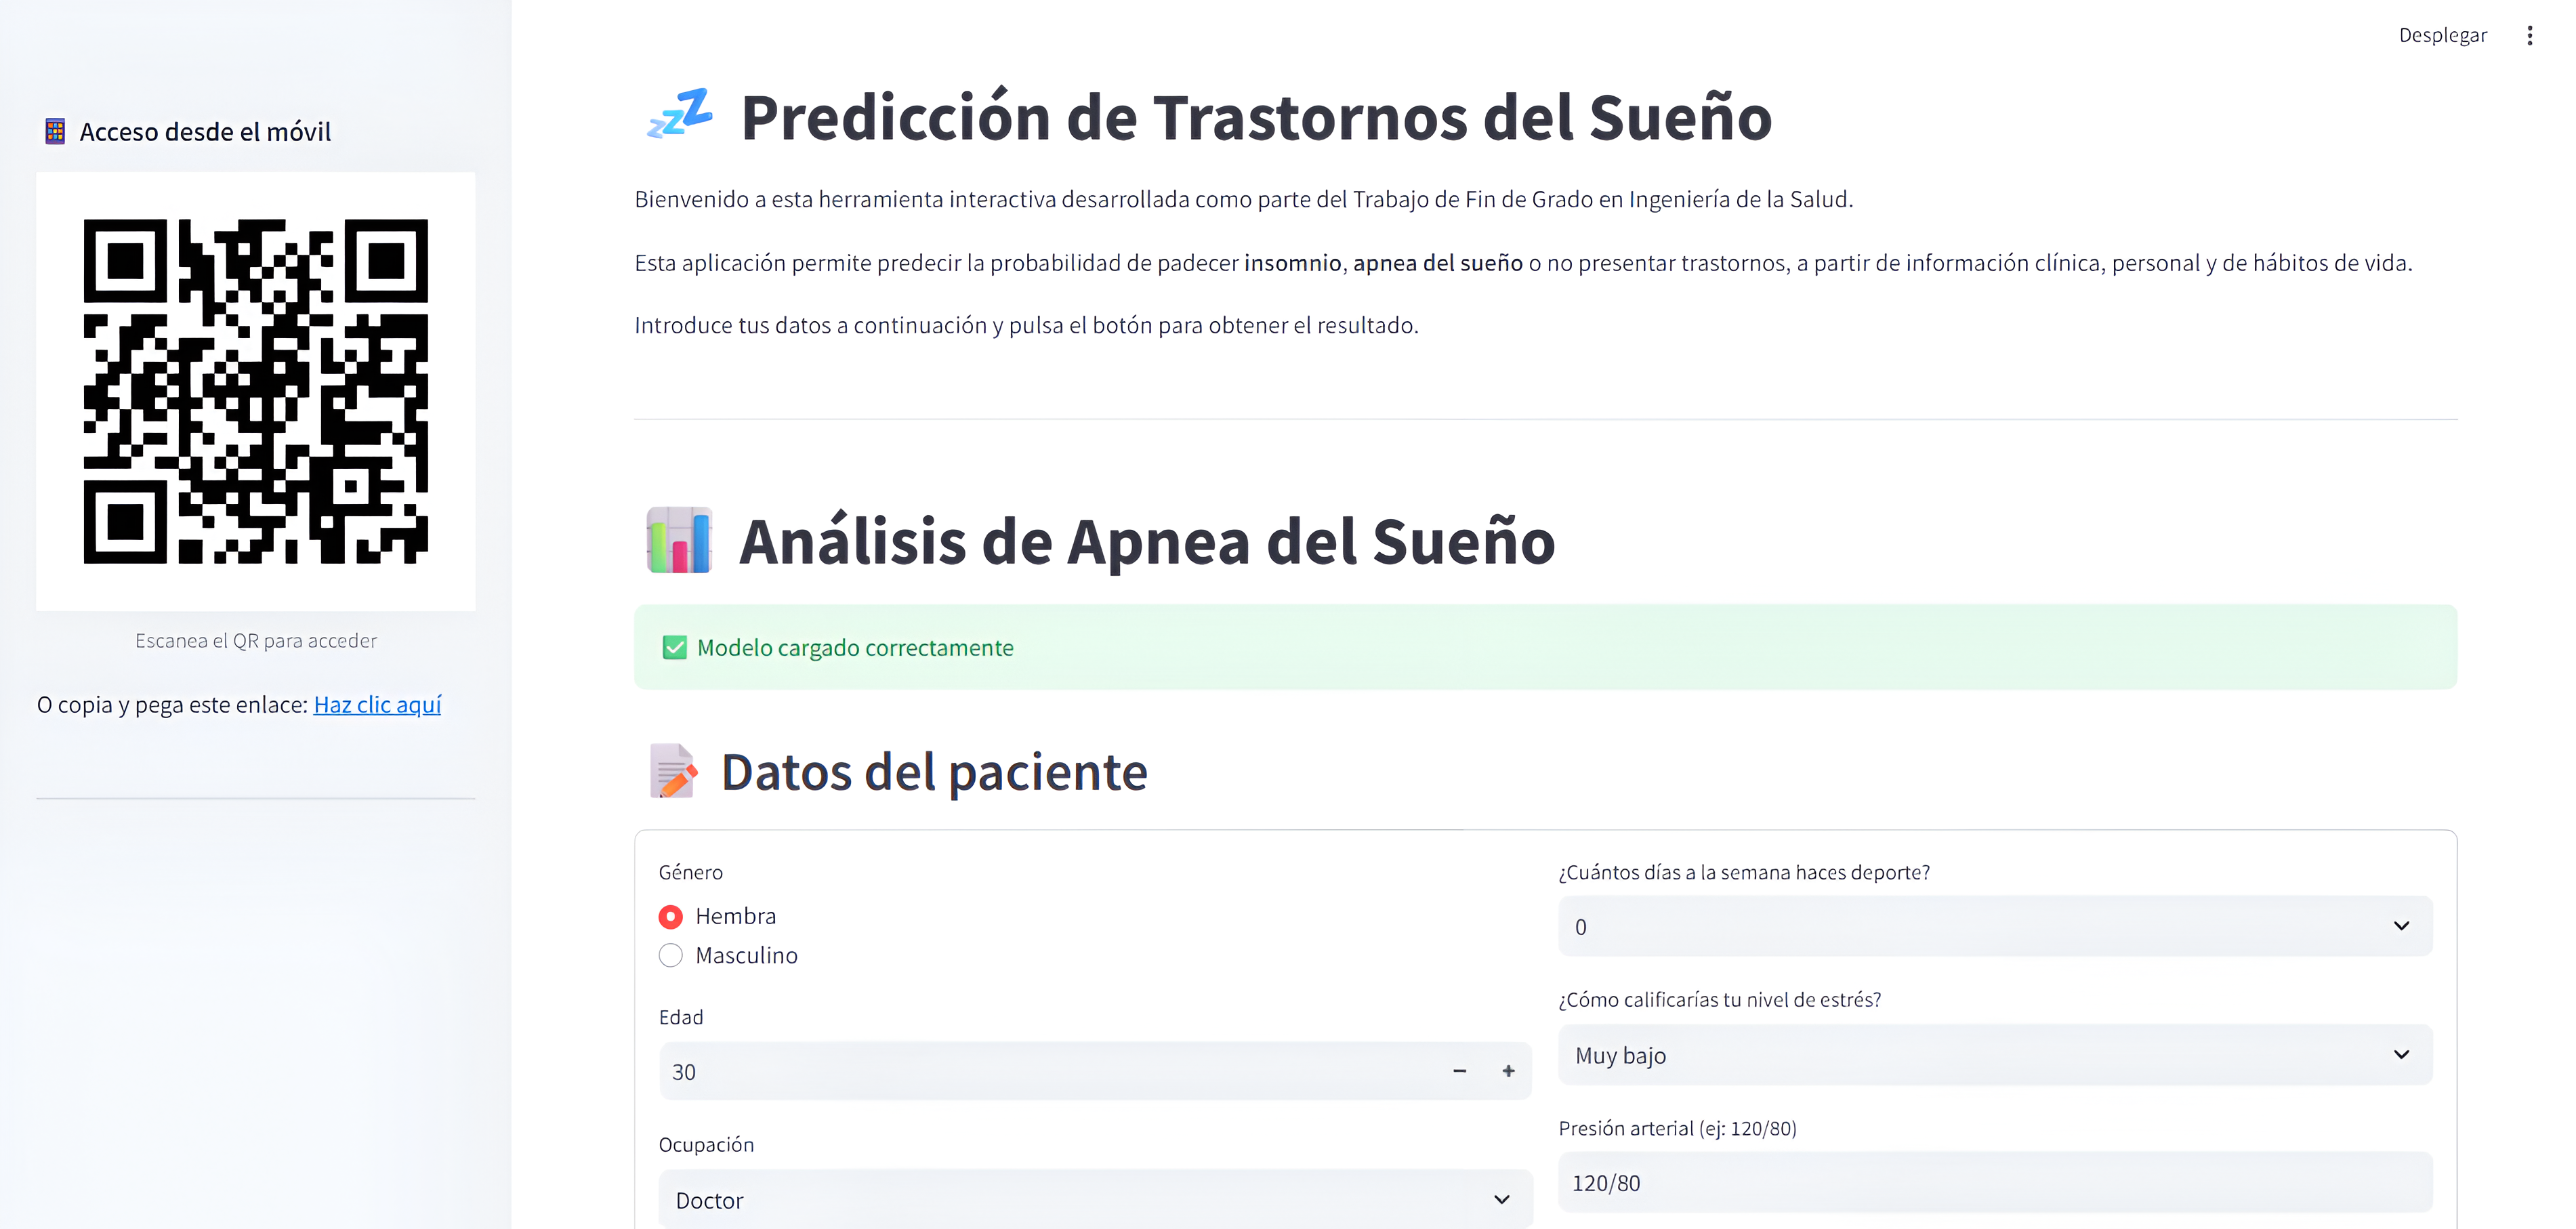
\includegraphics[width=1\linewidth]{img/interfazApp.png}
    \caption{Captura de la interfaz de la aplicación desarrollada en Streamlit.}
\end{figure}

\begin{figure}[H]
    \centering
    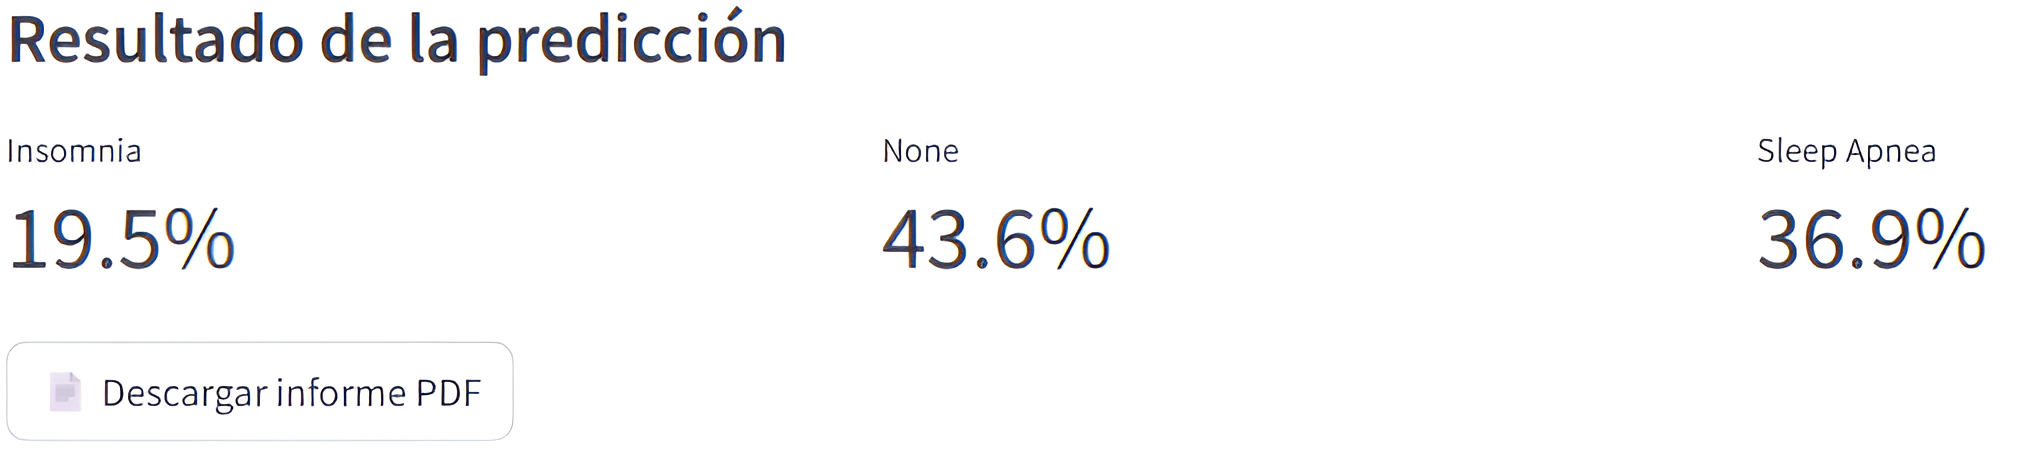
\includegraphics[width=0.9\textwidth]{img/resultadoPredd.png}
    \caption{Visualización de predicción.}
\end{figure}

\begin{figure}[H]
    \centering
    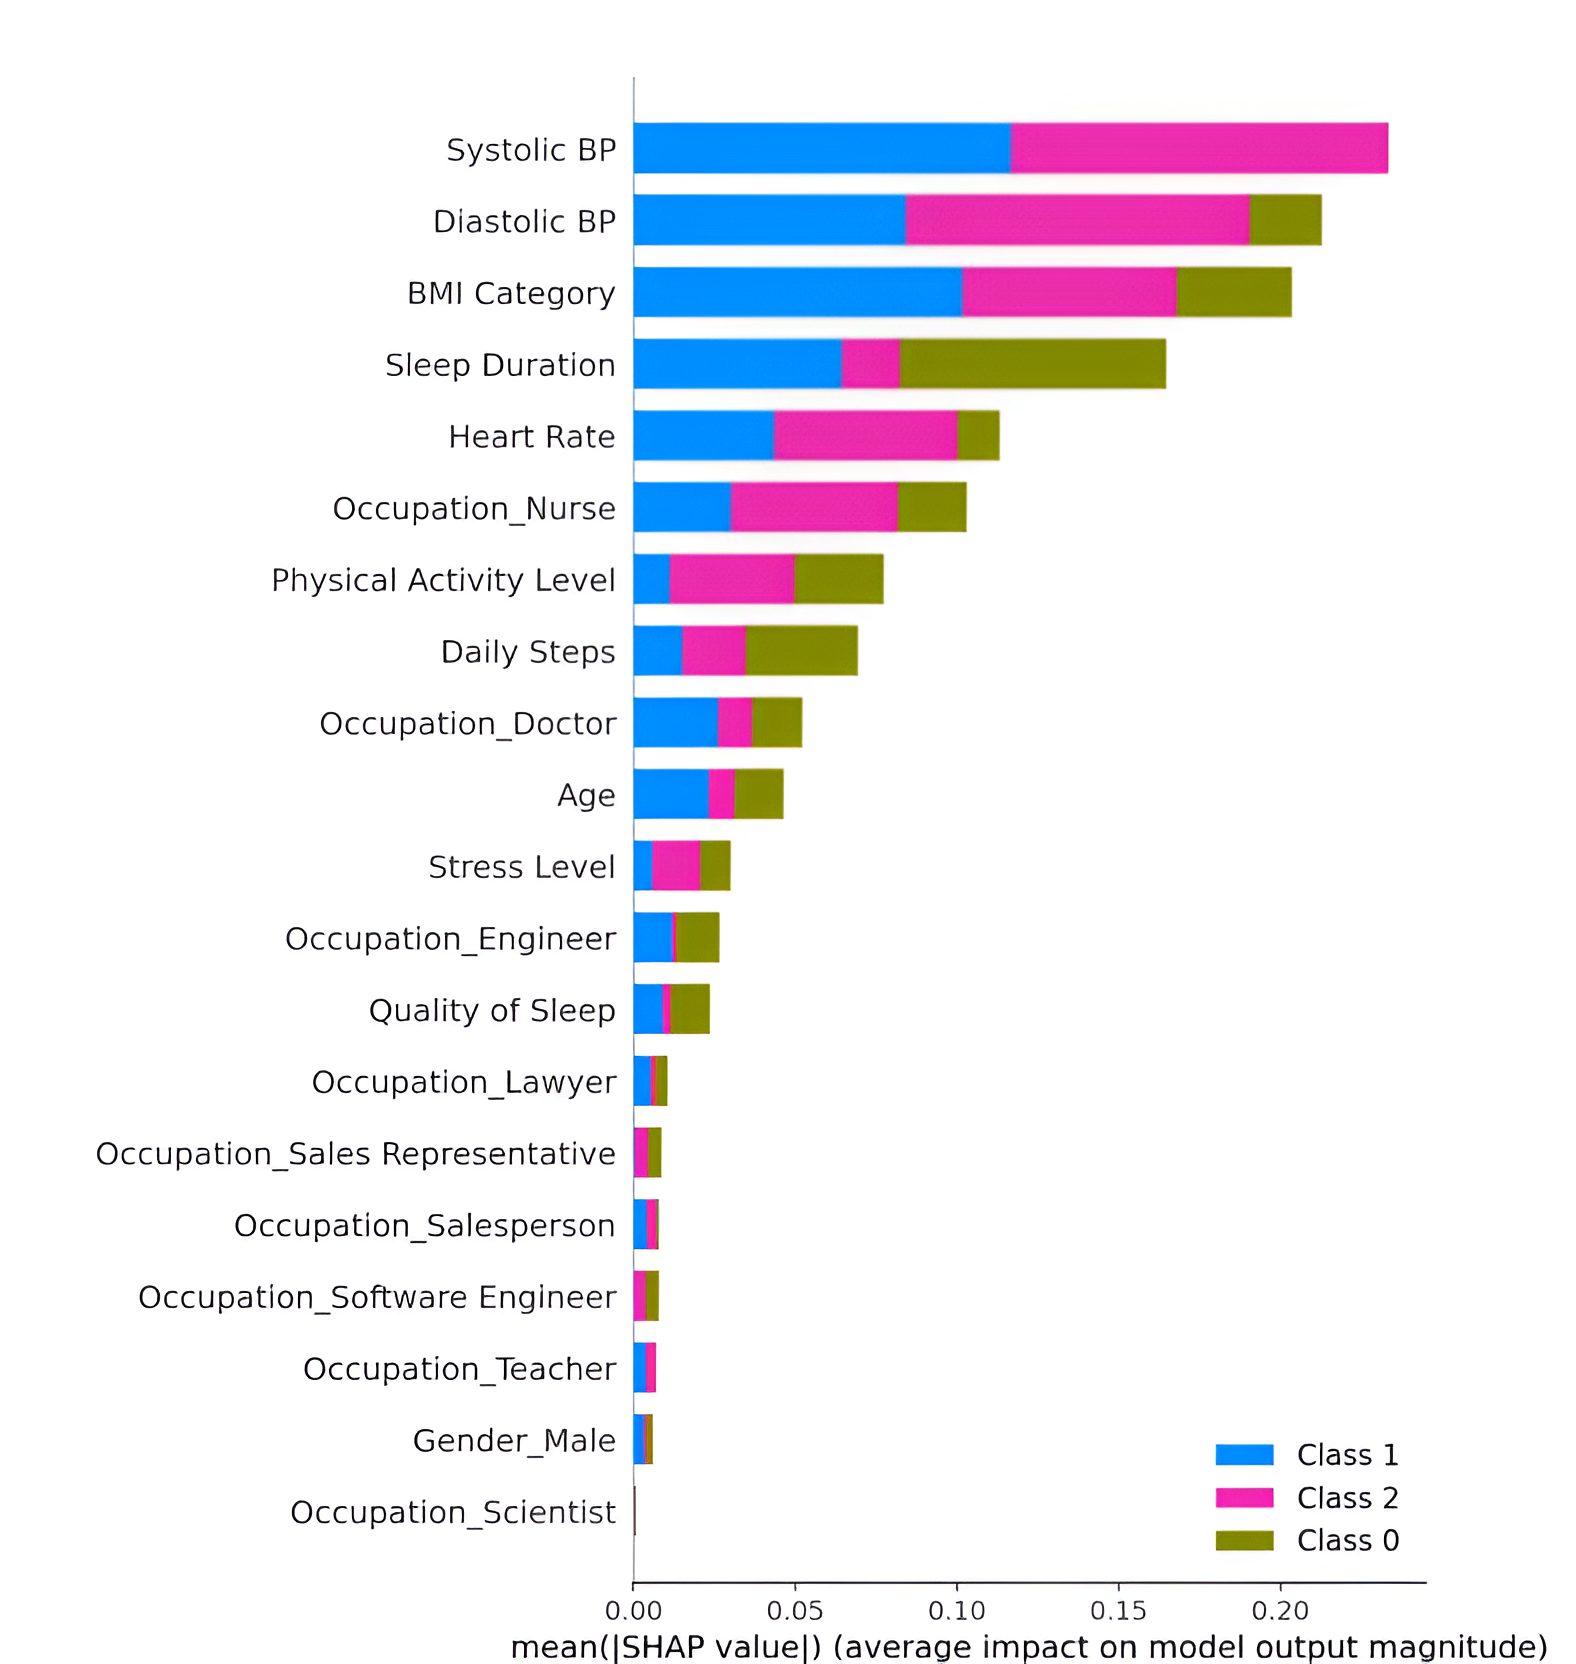
\includegraphics[width=0.75\linewidth]{img/shapApp.png}
    \caption{Explicación SHAP global en la interfaz.}
    \label{fig:shap}
\end{figure}


\begin{figure}[H]
    \centering
    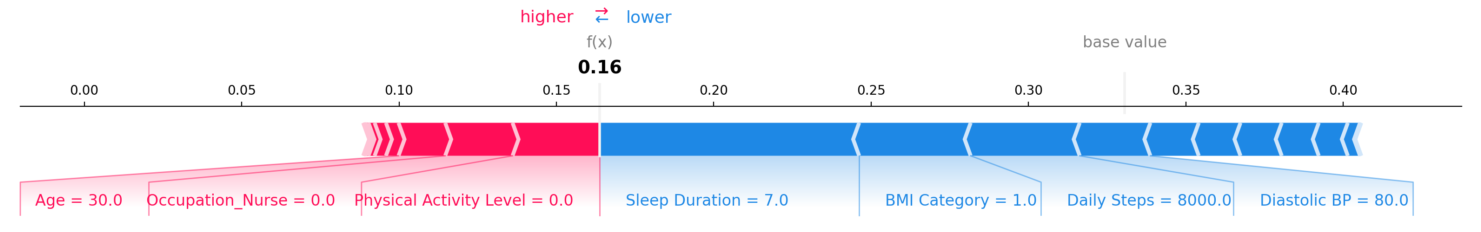
\includegraphics[width=1\linewidth]{img/explic_individual.png}
    \caption{Explicación SHAP individual.}
    \label{fig:shap}
\end{figure}


\section{Diseño de perfiles clínicos y validación externa}

Además de evaluar el rendimiento cuantitativo mediante métricas y representaciones gráficas, se consideró fundamental validar el sistema de forma práctica en situaciones clínicas. Para ello, se seleccionaron tres personas con características representativas de los tres grupos contemplados en la variable objetivo: pacientes con insomnio, con apnea del sueño y sin trastornos del sueño.

Estas personas fueron escogidas manualmente siguiendo criterios clínicos extraídos de la literatura científica y guías médicas sobre los principales factores de riesgo asociados a cada trastorno del sueño. A cada una se le colocó el dispositivo O2Ring para registrar sus variables fisiológicas reales, las cuales fueron posteriormente introducidas en la aplicación para comprobar la respuesta del modelo ante perfiles clínicamente relevantes.


\begin{itemize}
    \item \textbf{Factores de riesgo para Insomnio:} nivel de estrés elevado, mala calidad del sueño, duración inferior a 6 horas, baja actividad física, consumo de sustancias estimulantes, horarios de sueño irregulares y antecedentes de ansiedad o trastornos del estado de ánimo \cite{nhlbi_insomnio}.
    
    \item \textbf{Factores de riesgo para Apnea del Sueño:} obesidad, IMC elevado, hipertensión arterial, edad avanzada, género masculino, circunferencia de cuello grande, ronquidos, somnolencia diurna excesiva y estilo de vida sedentario \cite{mayoclinic_apnea}.

    \item \textbf{Factores asociados a un perfil sano:} sueño de buena calidad y duración ($\geq$ 7 horas), bajo nivel de estrés, presión arterial y frecuencia cardíaca dentro de rangos normales, actividad física alta y peso saludable.
\end{itemize}

El objetivo fue comprobar si el modelo asignaba correctamente la clase correspondiente a cada perfil clínico, reforzando así su coherencia médica en contextos clínicos reales.

\subsection{Validación externa con datos reales del dispositivo O2Ring}

Además de los tres perfiles seleccionados, se empleó un informe real del dispositivo biométrico \textbf{O2Ring}, utilizado habitualmente para el cribado domiciliario de trastornos respiratorios del sueño. El objetivo era comprobar si el sistema respondía adecuadamente ante un perfil clínico real compatible con apnea del sueño.

El informe generado por el O2Ring incluye indicadores como la saturación de oxígeno (SpO$_2$), la frecuencia cardíaca y métricas derivadas como:

\begin{itemize}
  \item \textbf{ODI 3\% y 4\% (Oxygen Desaturation Index)}: mide cuántas veces por hora la saturación de oxígeno desciende un 3\% o un 4\% respecto al valor basal. Valores superiores a 30 eventos/hora se consideran indicativos de apnea del sueño de grado grave, según los criterios clínicos establecidos por la literatura especializada \cite{zinchuk2018osa}.

  \item \textbf{Tiempo con SpO\textsubscript{2} < 90\%}: refleja la duración en la que el paciente estuvo en hipoxemia, siendo un indicador relevante en el diagnóstico de apnea y su gravedad.

  \item \textbf{Puntuación O2}: puntuación cualitativa que resume el comportamiento respiratorio nocturno (por ejemplo, la puntuación 3.0 implica riesgo alto).

  \item \textbf{SpO\textsubscript{2} mínima y promedio}: valores extremos de saturación durante la noche, útiles para detectar eventos severos.
\end{itemize}

En la literatura especializada, el ODI es una métrica aceptada como sustituto del índice de apneas-hipopneas (IAH) en entornos donde no se dispone de polisomnografía completa \cite{zinchuk2018osa}.

Aunque la aplicación desarrollada no se conecta directamente al O2Ring, se introdujo un perfil manual con características clínicas coherentes con el informe, lo que permitió comprobar si el modelo predecía correctamente la clase de apnea del sueño. En la Figura~\ref{fig:informeO2Ring} se muestra una captura del informe real empleado para esta validación.

\begin{figure}[H]
    \centering
    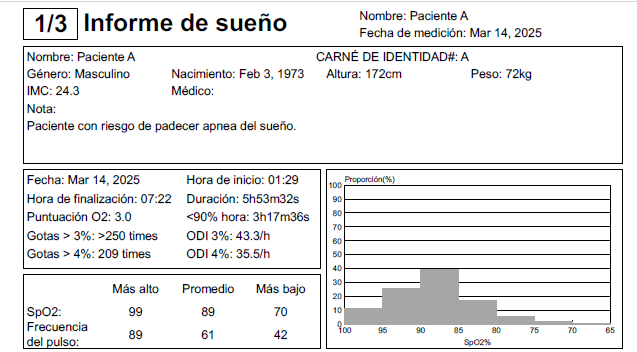
\includegraphics[width=0.85\textwidth]{img/informeSueño.png}
    \caption{Resumen del informe de sueño del dispositivo O2Ring para un caso compatible con apnea moderada.}
    \label{fig:informeO2Ring}
\end{figure}


\section{Técnicas y herramientas}

Esta sección recoge las herramientas de programación, bibliotecas y plataformas utilizadas para desarrollar el sistema predictivo y su despliegue en una aplicación web funcional. Se incluyen también referencias a los entornos de desarrollo y sistemas de documentación empleados, justificando su elección en función de su adecuación técnica al contexto sanitario y computacional del sistema.

\subsection{Python}

Python es un lenguaje de programación interpretado, de alto nivel y de propósito general, ampliamente utilizado en ciencia de datos, inteligencia artificial y desarrollo web. Su sintaxis sencilla, estructura modular y ecosistema de bibliotecas especializadas lo convierten en una herramienta ideal para proyectos de análisis de datos en entornos clínicos.

En este proyecto, Python se ha utilizado como lenguaje base para implementar todo el flujo de trabajo: desde la carga y el preprocesamiento de los datos hasta el entrenamiento, validación, calibración e interpretación del modelo. Además, permitió la construcción de la aplicación web interactiva mediante el framework Streamlit, así como la generación automática de informes en PDF. Su versatilidad ha sido clave para integrar, de forma eficiente y coherente, las diferentes fases del sistema desarrollado \cite{python2024}. 


\subsection{Jupyter Notebook}

Jupyter Notebook es una aplicación web de código abierto que permite crear y compartir documentos interactivos que combinan código ejecutable, visualizaciones, fórmulas matemáticas y texto explicativo. Está especialmente diseñada para entornos de ciencia de datos, aprendizaje automático y análisis computacional, y se ha convertido en una herramienta estándar en investigación y docencia.

Aunque admite múltiples lenguajes de programación mediante el uso de kernels, su integración con Python es la más extendida. Una de sus principales ventajas es la posibilidad de estructurar el trabajo en celdas independientes, lo que permite ejecutar fragmentos de código por separado, visualizar resultados en tiempo real e ir documentando el proceso paso a paso. Esto facilita la validación iterativa, el análisis exploratorio de datos y la depuración eficiente del flujo de trabajo.

En el presente proyecto, Jupyter Notebook se utilizó durante las fases de exploración, preprocesamiento, entrenamiento del modelo y visualización de resultados. Su entorno interactivo ha permitido documentar el desarrollo de forma ordenada, facilitando tanto el análisis como la futura reproducibilidad del sistema construido. \cite{jupyter2024}


\subsection{Anaconda Navigator}

Anaconda es una distribución de código abierto ampliamente utilizada en entornos científicos y de ciencia de datos, ya que facilita la instalación y gestión de entornos virtuales, paquetes y dependencias en Python. Incorpora más de 250 bibliotecas populares preinstaladas, incluyendo \texttt{Pandas}, \texttt{NumPy}, \texttt{scikit-learn}, \texttt{matplotlib} y muchas otras, lo que agiliza el proceso de configuración del entorno de desarrollo.

Dentro de esta distribución, \textbf{Anaconda Navigator} actúa como una interfaz gráfica que permite gestionar entornos, lanzar herramientas como Jupyter Notebook, Spyder o VSCode, e instalar nuevas bibliotecas sin necesidad de comandos en terminal. Esta facilidad de uso lo convierte en una herramienta ideal para proyectos multidisciplinares, especialmente en contextos como la ingeniería de la salud, donde se busca acelerar el desarrollo y garantizar la reproducibilidad.

En este proyecto se utilizó Anaconda para gestionar el entorno de trabajo, instalar todas las dependencias necesarias y organizar los paquetes empleados en las fases de análisis, modelado e implementación de la aplicación. \cite{anaconda2024}


\subsection{Pandas y Numpy}
Pandas es una biblioteca de Python especializada en la manipulación y análisis de datos en estructuras tabulares. Permite trabajar con objetos de tipo \texttt{DataFrame}, que representan conjuntos en formato fila-columna similar a una hoja de cálculo o una tabla SQL. Esta herramienta facilita tareas como la lectura de archivos, limpieza de datos, conversión de tipos...

En este proyecto, Pandas se utilizó en todas las fases del tratamiento de datos: desde la carga inicial del conjunto en formato CSV hasta la transformación de variables, el análisis exploratorio y la preparación del dataset para su posterior entrada al modelo.

Por otro lado, \textbf{Numpy} es una librería orientada al cálculo científico. Proporciona una estructura eficiente para trabajar con \textbf{arrays multidimensionales}, además de incluir funciones matemáticas y estadísticas vectorizadas de alto rendimiento. Fue utilizada de forma complementaria para operaciones aritméticas sobre columnas numéricas y para asegurar un procesamiento rápido y preciso de datos a gran escala.

\subsection{SHAP}

\textbf{SHAP} (SHapley Additive exPlanations) es una librería de Python que permite interpretar modelos de aprendizaje automático complejos mediante la teoría de los valores de Shapley, desarrollada en el marco de los juegos cooperativos. Esta técnica asigna a cada variable una contribución cuantitativa al resultado de una predicción, permitiendo explicar de forma transparente cómo se ha llegado a una determinada clasificación.

En el presente proyecto, SHAP se utilizó para analizar el modelo final (Random Forest) desde dos enfoques complementarios: global e individual. A nivel global, se generaron gráficos resumen (\textit{summary plots}) que muestran la importancia media de cada variable en todas las predicciones. A nivel individual, se aplicaron \textit{force plots} que descomponen la predicción para un usuario específico, visualizando cómo cada variable influye positiva o negativamente en el resultado.

La incorporación de SHAP ha sido clave para garantizar la interpretabilidad del sistema, un aspecto esencial en contextos relacionados con la salud, donde es necesario justificar cada decisión automatizada de forma comprensible y clínicamente relevante.

\subsection{Matplotlib y Seaborn}

\textbf{Matplotlib} y \textbf{Seaborn} son bibliotecas de visualización de datos en Python que permiten generar gráficos personalizados con gran control sobre el estilo y la presentación. Matplotlib proporciona una base versátil para construir figuras a bajo nivel, mientras que Seaborn ofrece una capa de abstracción más sencilla para crear visualizaciones estadísticas complejas con menos código.

Estas herramientas se emplearon en las fases de análisis exploratorio de datos (EDA), visualización de correlaciones, detección de valores atípicos y representación gráfica de resultados. Entre las visualizaciones generadas se encuentran histogramas, gráficos de densidad (KDE), diagramas de caja y violín, mapas de calor (\textit{heatmaps}), matrices de confusión y gráficos de importancia de variables.


\subsection{Streamlit}

Streamlit es un framework de código abierto diseñado para crear aplicaciones web interactivas directamente desde scripts de Python, sin necesidad de conocimientos en desarrollo frontend. Permite transformar scripts de análisis y modelos predictivos en interfaces web funcionales con muy poco código adicional, lo que lo convierte en una herramienta ideal para proyectos de ciencia de datos aplicada y prototipos clínicos.

Entre sus principales ventajas se encuentran la facilidad de uso, su compatibilidad con bibliotecas populares como \texttt{Pandas}, \texttt{scikit-learn} y \texttt{matplotlib}, y la capacidad de actualizar resultados en tiempo real conforme el usuario introduce nuevos datos.

En este proyecto, Streamlit se empleó para construir una aplicación web interactiva que permite al usuario introducir datos clínicos y de estilo de vida, generar una predicción automática sobre el trastorno del sueño más probable, y visualizar una explicación personalizada del resultado mediante gráficos de SHAP. La herramienta fue desplegada en la nube mediante \textit{Streamlit Community Cloud}, garantizando su accesibilidad desde cualquier navegador sin necesidad de instalación. \cite{streamlit}


\subsection{FPDF}
\textbf{FPDF} es una librería de código abierto utilizada para la creación de archivos PDF desde scripts de Python. Gracias a su flexibilidad de diseño y sintaxis intuitiva permite generar informes personalizados y documentos portables.

En el presente proyecto, FPDF fue empleada dentro de la aplicación web interactiva para construir informes automáticos. Estos documentos resumen los datos introducidos por el usuario, la predicción generada por el modelo y una representación visual explicativa basada en SHAP. El objetivo fue proporcionar al usuario un documento descargable que pueda guardar, imprimir o compartir, facilitando así la continuidad del seguimiento clínico o la consulta posterior.

\subsection{Visual Studio}

\textbf{Visual Studio Code} (VS Code) es un entorno de desarrollo integrado (IDE) de código abierto desarrollado por Microsoft. Se caracteriza por su ligereza, extensibilidad y compatibilidad multiplataforma. Permite programar en múltiples lenguajes, entre ellos Python, C++, JavaScript y C\#, y ofrece funcionalidades como resaltado de sintaxis, autocompletado inteligente, depuración paso a paso, control de versiones mediante Git y terminal integrada.

Durante el desarrollo de este proyecto, VS Code fue utilizado como entorno principal para organizar los scripts en Python, estructurar la lógica de predicción, integrar la aplicación en Streamlit y realizar pruebas funcionales del sistema. Su compatibilidad con entornos virtuales, su integración con GitHub y su interfaz modular facilitaron un flujo de trabajo limpio, ordenado y eficiente.

\subsection{GitHub}
\textbf{GitHub} es una plataforma para el control de versiones y la gestión de proyectos basada en el sistema Git. Permite almacenar, organizar y versionar el código fuente de forma colaborativa, además de ofrecer herramientas para documentación, seguimiento de cambios y despliegue de aplicaciones.

En este proyecto, GitHub fue utilizado como repositorio central para el código del modelo, los scripts de preprocesamiento y la implementación de la aplicación web. Gracias a este sistema se garantizó la trazabilidad del desarrollo, la seguridad frente a pérdidas accidentales de información y la posibilidad de reproducir el trabajo completo en futuros entornos.

\subsection{LaTex (Overleaf)}
\textbf{LaTeX} es un sistema de composición tipográfica de alta calidad, ampliamente utilizado en la redacción de documentos técnicos y científicos. Permite estructurar contenidos con precisión, insertar fórmulas matemáticas complejas, generar índices automáticos y gestionar bibliografía de forma eficiente.

Para la redacción de esta memoria se ha utilizado la plataforma \textbf{Overleaf}, un editor LaTeX en línea que permite la escritura colaborativa, el seguimiento de versiones y la integración de paquetes personalizados. Esta herramienta ha sido clave para presentar los contenidos del trabajo con claridad, rigor formal y formato profesional, incluyendo gráficos, referencias cruzadas y citación bibliográfica automatizada.

\subsection{O$_2$ Insight Pro}

\textbf{O$_2$ Insight Pro} es el software oficial del dispositivo portátil \textit{O2Ring} (Viatom), utilizado para visualizar, analizar y exportar datos fisiológicos registrados durante el sueño. Este programa permite extraer variables como la saturación de oxígeno (SpO$_2$), la frecuencia cardíaca, el número de eventos de desaturación y el índice ODI.

Aunque no formó parte del sistema implementado, se utilizó durante la fase de validación externa para obtener registros reales de pacientes y comprobar el comportamiento del modelo ante casos clínicos simulados. Los datos exportados desde O$_2$ Insight Pro se integraron manualmente en el conjunto de entrada de la aplicación, permitiendo una comparación cualitativa entre predicción y perfil fisiológico real.